\chapter{Applications}
\label{chap:applications}

\begin{figure}[ht]
	\hfill
	\begin{minipage}{0.5\textwidth}
		\centering
		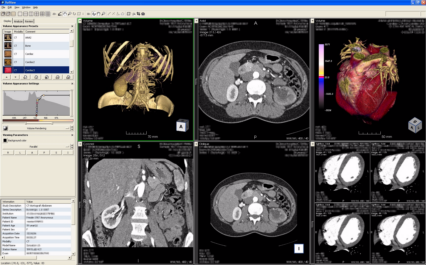
\includegraphics{VTKTextbook-275}
		\caption*{\texttt{Streamline visualization with ParaView Enterprise Edition.}}
	\end{minipage}
\end{figure}


\firstletter{W}e have described the design and implementation of an extensive toolkit of visualization techniques.
In this chapter we examine several case studies to show how to use these tools to gain insight into important application areas.
These areas are medical imaging, financial visualization, modeling, computational fluid dynamics, finite element analysis, and algorithm visualization. For each case, we briefly describe the problem domain and what information we expect to obtain through visualization.
Then we craft an approach to show the results.
Many times we will extend the functionality of the Visualization Toolkit with application specific tools.
Finally, we present a sample program and show resulting images.
The visualization design process we go through is similar in each case.
First, we read or generate application-specific data and transform it into one of the data representation types in the Visualization Toolkit.
Often this first step is the most difficult one because we have to write custom computer code, and decide what form of visualization data to use.
In the next step, we choose visualizations for the relevant data within the application.
Sometimes this means choosing or creating models corresponding to the physical structure. Examples include spheres for atoms, polygonal surfaces to model physical objects, or computational surfaces to model flow boundaries.
Other times we generate more abstract models, such as isosurfaces or glyphs, corresponding to important application data.
In the last step we combine the physical components with the abstract components to create a visualization that aids the user in understanding the data.

\section{3D Medical Imaging}
Radiology is a medical discipline that deals with images of human anatomy.
These images come from a variety of medical imaging devices, including X-ray, X-ray Computed Tomography (CT), Magnetic Resonance Imaging (MRI), and ultrasound. Each imaging technique, called an imaging modality, has particular diagnostic strengths.
